\documentclass{article}
% =======PACKAGES=======
% FORMATTING
\usepackage[margin=0.625in]{geometry}
\usepackage{parskip, setspace}
\setstretch{1.15}
% TYPESETTING - MATH
\usepackage{amsmath, amsfonts}
\usepackage{amsthm}
\usepackage[ruled, linesnumbered, noend]{algorithm2e}
\NewCommandCopy{\legacyunderscore}{\_}
\renewcommand{\_}{\ifincsname_\else\legacyunderscore\fi}
\usepackage{listings}
\usepackage{xcolor}
\usepackage{algorithm2e}

\lstdefinestyle{mystyle}{
    backgroundcolor=\color{lightgray},   
    commentstyle=\color{darkgray},
    keywordstyle=\color{red},
    numberstyle=\color{black},
    stringstyle=\color{violet},
    basicstyle=\ttfamily\footnotesize,
    breakatwhitespace=false,         
    breaklines=true,                 
    captionpos=b,                    
    keepspaces=true,                 
    numbers=left,                    
    numbersep=5pt,                  
    showspaces=false,                
    showstringspaces=false,
    showtabs=false,                  
    tabsize=2
}
\lstset{style=mystyle}
% RICH
\usepackage{graphicx, caption}
\usepackage{hyperref}
% BIBLIOGRAPHY
\usepackage[
backend=biber,
sorting=ynt
]{biblatex}
\addbibresource{bib.bib}

\newcommand{\integer}{\textbf{int} }

% =======TITLE=======
\title{\vspace*{-0.625in}CS 529: Advanced Data Structures \& Algorithms \\ Assignment 7: Johnson-Lindenstrauss and Monotone Boolean Functions}
\author{Nathan Chapman, Hunter Lawrence, Andrew Struthers}
\date{\today}

\begin{document}

\maketitle

\section*{Summary of Johnson-Lindenstrauss Lemma}

The Johnson-Lindenstrauss lemma is a fundamental result in mathematics and computer science that deals with dimensionality reduction. Named after William B. Johnson and Joram Lindenstrauss, who independently proved it in the 1980s, the lemma addresses the problem of preserving the pairwise distances between points in high-dimensional Euclidean space while projecting them into lower-dimensional spaces.

The lemma states that for any set of points in a high-dimensional Euclidean space, there exists a low-dimensional subspace onto which the points can be efficiently and linearly mapped, such that the pairwise distances between the points are approximately preserved. Specifically, for any $\epsilon > 0$ and any integer $n$, given a set of $m$ points in high-dimensional space (originally in $\mathbb{R}^d$), there exists a mapping to a lower-dimensional space ($\mathbb{R}^k$, where $k$ is significantly smaller than $d$) such that the distances between any pair of points are preserved up to a factor of $(1 \pm \epsilon)$.

\begin{enumerate}
    \item \textbf{Efficiency}: The lemma assures us that such a mapping can be constructed efficiently, meaning that it doesn't require excessive computational resources even for large datasets.
    
    \item \textbf{Applications in Machine Learning and Data Mining}: The Johnson-Lindenstrauss lemma has numerous applications in machine learning and data mining. It is particularly useful in dimensionality reduction techniques like Principal Component Analysis (PCA), t-distributed Stochastic Neighbor Embedding (t-SNE), and Locally Linear Embedding (LLE). By reducing the dimensionality of data, these techniques help in visualizing and understanding high-dimensional datasets, while still preserving the essential geometric structure and relationships between data points.
    
    \item \textbf{Sparse Signal Processing}: In signal processing, especially in sparse signal processing, where signals are often represented in high-dimensional spaces, the lemma finds applications in compressive sensing. It enables the reconstruction of sparse signals from a small number of linear measurements by projecting them onto a lower-dimensional space while preserving their structure.
    
    \item \textbf{Nearest Neighbor Search}: Another significant application is in nearest neighbor search algorithms. By reducing the dimensionality of the feature space, the computational complexity of searching for nearest neighbors is greatly reduced while maintaining the accuracy of the search.
    
    \item \textbf{Big Data Analysis}: With the rise of big data, the Johnson-Lindenstrauss lemma provides a powerful tool for dealing with high-dimensional datasets efficiently. It allows for the analysis of large-scale datasets without sacrificing the quality of results.
\end{enumerate}

\begin{figure}[h]
    \centering
    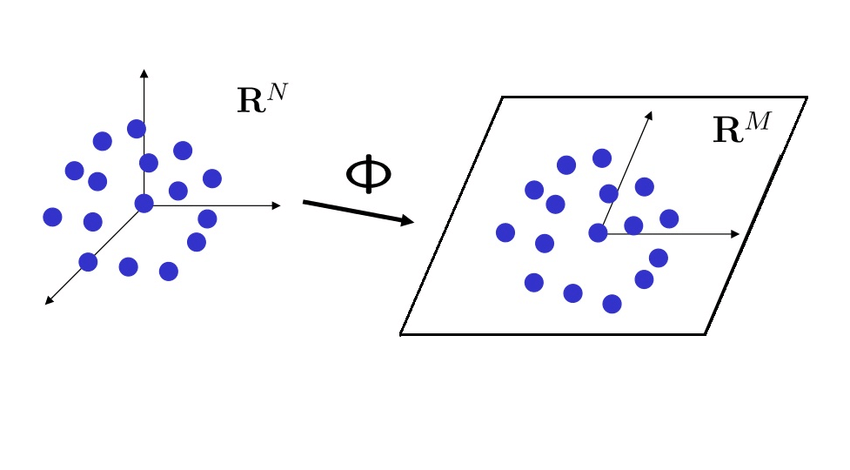
\includegraphics[width=0.5\textwidth]{dimensionality_reduction.png}
    \caption{Visualization of Dimensionality Reduction}
    \label{fig:dimensionality_reduction}
\end{figure}
\newpage

The Johnson-Lindenstrauss lemma is important in machine learning, data mining, signal processing, and big data analysis by providing a way to reduce the dimensionality of data while preserving its inherent structure and relationships.


\section*{Minimal Dimension Reduction}

    Estimate the minimal dimsension $k$ to preserve n-D distances of 20 arbitrary n-D points within $\pm5\%$ and $\pm50\%$ accuracy.

    \underline{\textbf{Solution}}

    The Johnson-Lindenstrauss lemma can be stated as 

    \begin{quote}
        For any $\epsilon \in (0,1)$ and any integer $n \geq 15(\log m) / \epsilon^2$, there exists a linear function $f: \mathbb{R}^N \to \mathbb{R}^n$ such that the restriction $f|_X$ is $(1 + \epsilon)$-bi-Lipschitz.
    \end{quote}

    We can equate this notation to our notation as

    \begin{itemize}
        \item The reduced dimension: $n = k$
        \item The size of the collection of points: $m = 20$
        \item The percent accuracy: $\epsilon = 5$ or $\epsilon = 50$.
    \end{itemize}

    Additionally, the minimal dimension that preserves such accuracy is when $n = \lceil 15(\log m) / \epsilon^2 \rceil$. Therefore, the minimal dimension $k$ that preserves distance with in $\pm\epsilon\%$ for a collection of 20 points is 

    \begin{subequations}
        \begin{equation*}
            k_5 = \left\lceil \frac{15 (\log 20)}{5^2} \right\rceil = 9
        \end{equation*}
        \begin{equation*}
            k_{50} = \left\lceil \frac{15 (\log 20)}{50^2} \right\rceil = 1
        \end{equation*}    
    \end{subequations}
    

\section*{Summary of Restoration of Monotone Boolean Functions}
Optimal restoration of monotone Boolean functions is a significant problem in computer science, particularly in the field of Boolean function analysis and optimization. Monotone Boolean functions are functions that only increase or stay the same as their inputs increase. The optimal restoration problem involves finding the minimal set of variables to restore in a given faulty Boolean function to make it monotone again. This problem has implications in circuit design, fault tolerance, reliability analysis, and error correction in digital systems.

The optimal restoration of monotone Boolean functions problem aims to identify the smallest subset of variables in a faulty Boolean function that, when restored (or fixed), render the function monotone. Given a faulty Boolean function that has become non-monotone due to some faults or errors in its variables, the objective is to determine the minimum number of variable fixes needed to restore the monotonicity of the function.

Formally, for a given monotone Boolean function \( f \) with inputs \( x_1, x_2, \ldots, x_n \), and a set of faulty variables \( F \subseteq \{x_1, x_2, \ldots, x_n\} \), the goal is to find the smallest subset \( R \subseteq F \) such that the function becomes monotone when the variables in \( R \) are restored to their original values.

This problem has been extensively studied in the context of fault-tolerant circuit design, where ensuring monotonicity is crucial for correct circuit behavior, especially in critical applications such as safety-critical systems and aerospace engineering.

\begin{enumerate}
    \item \textbf{Algorithmic Approaches}: Several algorithmic approaches have been proposed to solve the optimal restoration problem efficiently. These approaches often leverage properties of monotone Boolean functions and employ techniques such as dynamic programming, branch-and-bound algorithms, and greedy algorithms to identify the minimal restoration set.
    
    \item \textbf{Complexity Analysis}: The optimal restoration problem is known to be NP-hard, as it involves finding the smallest subset of variables that satisfies a specific property (monotonicity) in a Boolean function. As a result, heuristic and approximation algorithms are commonly used to tackle large instances of the problem.
    
    \item \textbf{Applications in Circuit Design}: In digital circuit design, ensuring the monotonicity of Boolean functions is crucial for maintaining reliable and predictable behavior. The optimal restoration problem helps in identifying and correcting faults in circuits to prevent non-monotonic behavior, which can lead to incorrect operation or even system failure.
    
    \item \textbf{Fault Tolerance and Reliability Analysis}: Monotone Boolean functions are used in modeling various aspects of fault-tolerant systems and reliability analysis. By studying the optimal restoration problem, researchers can develop techniques to enhance the fault tolerance and reliability of digital systems by efficiently identifying and correcting faults.
    
    \item \textbf{Error Correction in Digital Systems}: In addition to fault tolerance, the optimal restoration problem has implications for error correction in digital systems. By restoring non-monotone functions to monotone ones, errors introduced during computation or communication can be mitigated, leading to improved system performance and accuracy.
\end{enumerate}
\begin{figure}[h]
    \centering
    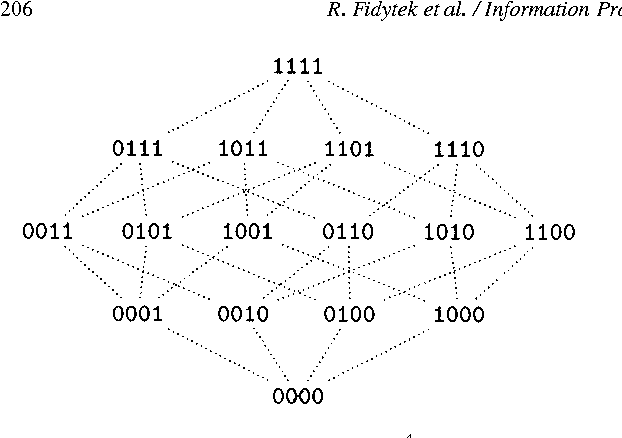
\includegraphics[width=0.75\textwidth]{Monotone_Boolean_functions}
    \caption{Visualization of a Boolean function}
    \label{fig:dimensionality_reduction}
\end{figure}
\newpage



\section*{Constructing Hansel Chains for Monotone Boolean Functions}

The first step required to restore a function is to construct a sorted list of Hansel Chains using the functions \\$createHanselChains()$. After this is completed, it is necessary to initialize $restoredFunctionValue$ to infinity so that even large values of the boolean function $f(x)$ will be caught when checking the chains for the function value.

From here, we reconstruct the function by checking for link heads that do not produce a positive result for $f(x)$, when one is found, it is iterated through until the smallest value in the chain that produces a positive value for $f(x)$ is found. This value is then converted to decimal and, if the vector's decimal value is less than $restoredFunctionValue$, is saved as the $restoredFunctionValue$. When this loop is completed, and all chain heads are checked, the value of $restoredFunctionValue$ will represent the function value for $f(x)$.

\begin{algorithm}[!h]
    \DontPrintSemicolon
    \caption{$generateBooleanFunction(f(x))$}
    \label{alg:sp500}
    \KwIn{A function to re-construct a given monotone boolean function $f(x)$ and the number of dimensions for the solution vectors $dimensions$}
    \KwOut{The function value to restore (assuming the boolean function returns true if above this value to restore)}
    \textbf{Assumes:} The presence of some function $getDecimalValue()$ which returns the decimal value of a binary vector.
    \BlankLine

    $hanselChains \gets createHanselChains(dimensions)$\\

    $restoredFunctionValue \gets \infty$\\\BlankLine

    $numChains \gets hanselChains.length()$\\\BlankLine

    $i \gets 0$\\
    \While{$i < numChains$}{

        // for each chain head that does not produce a positive value\\
        \If{$!f(hanselChains[i][0])$}{
            // find the first (lowest) index that will produce a 1\\
            $chainLength \gets hanselChains[i].length()$\\\BlankLine

            $j \gets 0$\\
            \While{$j < hanselChains[i].length()$}{
                \If{$f(hanselChains[i][j])$}{
                    // if the current vector is less than the best so far, save it as $restoredFunctionValue$\\\BlankLine

                    \If{$hanselChains[i][j].getDecimalValue() < restoredFunctionValue$}{
                        $restoredFunctionValue = hanselChains[i][j].getDecimalValue()$\\
                    }
                    
                }
                $j++$\\
            }
            
        }\BlankLine
        $i++$\\
    }

    \Return{$restoredFunctionValue$}
\end{algorithm} 




.

\begin{algorithm}[!h]
    \DontPrintSemicolon
    \caption{$createHanselChains(n)$}
    \label{alg:sp500}
    \KwIn{An integer $n$ representing the length of each boolean vector}
    \KwOut{An unsorted two dimensional list of Hansel Chains and the vectors in each}
    \textbf{Assumes:} The availability of some function $sort()$, which will sort chains based on the total value of their first vector in order from highest to lowest.
    \BlankLine
    
    $hanselChains \gets {<0, 1>}$
    
    $i \gets 1$

    \While{$i < n$}{
        $numChains \gets 2^(i-1)$\\\BlankLine
        // clone and grow all current chains\\
        $cloneAndGrowChains(hanselChains, numChains)$\\\BlankLine

        // cut and add to newly changed chains\\
        $cutAndAddChains(hanselChains, numChains)$\\\BlankLine

        $i++$\\
    }\BlankLine

    $hanselChains.sort()$

    \Return{$hanselChains$}
\end{algorithm} 



\begin{algorithm}[!h]
    \DontPrintSemicolon
    \caption{$cloneAndGrowChains(chains, numChains)$}
    \label{alg:sp500}
    \KwIn{A three dimensional array of chains $chains$, and a number of currently available chains $numChains$}
    \KwResult{Clones and grows present chains}
    \textbf{Assumes:} The presence of some function $clone()$ that copies an array, some function $insert(index, value)$ that places a $value$ at a provided index $index$ and shifts all other values right, and some function $add(value)$ that places a $value$ at the last index of an array.
    \BlankLine

    $i \gets 0$\\

    \While{$i < numChains$}{
        // clone each chain\\
        $newChain \gets chains[i].clone()$\\\BlankLine

        // grow each chain\\
        $newChain.insert(0, 0)$\\\BlankLine
        $chains[i].insert(0, 1)$\\

        $chains.add(newChain)$\\\BlankLine

        $i++$\\
    }

    \BlankLine
\end{algorithm} 




\begin{algorithm}[!h]
    \DontPrintSemicolon
    \caption{$cutAndAddChains(chains, numChains)$}
    \label{alg:sp500}
    \KwIn{A three dimensional array of chains $chains$, and a number of currently available chains $numChains$}
    \KwResult{Cuts and grows present chains}
    \textbf{Assumes:} The presence of some function $add(value)$ that places a $value$ at the last index of an array, some function $getLastIndex()$ which gets the last index of an array, some function $deleteLastIndex()$ which removes the last index of an array.
    \BlankLine

    $i \gets 0$\\

    \While{$i < numChains$}{
        // move the last vector from the clone chain to original chain\\
        $chains[i].add(chains[numChains+i].getLastIndex())$\\
        $chains[numChains+i].deleteLastIndex()$\\\BlankLine
        $i++$\\
    }
    \BlankLine
    
\end{algorithm} 


\end{document}